\experiment{Sorting Algorithms}{01/12/2023}

\section{Aim}
Implement the following sorting algorithms to sort a given set of elements in ascending order:
\begin{enumerate}
  \item Bubble Sort
  \item Selection Sort
  \item Insertion Sort
  \item Merge Sort
  \item Quick Sort
  \item Heap Sort
\end{enumerate}

\section{Algorithm}
 {\fontfamily{lmtt}\selectfont

  \subsection{Function: \texttt{display(arr, n)}}
  \begin{enumerate}[label*=\arabic*.]
    \item \textbf{Start}
    \item Loop from \texttt{i} equal to 0 to \texttt{n - 1}:
          \begin{enumerate}[label*=\arabic*.]
            \item Print \texttt{arr[i]} followed by a space.
          \end{enumerate}
    \item Print a newline.
    \item \textbf{Stop}
  \end{enumerate}

  \subsection{Function: \texttt{bubbleSort(arr, n)}}
  \begin{enumerate}[label*=\arabic*.]
    \item \textbf{Start}
    \item Loop from \texttt{i} equal to \texttt{n - 1} down to 0:
          \begin{enumerate}[label*=\arabic*.]
            \item Loop from \texttt{j} equal to 0 to \texttt{i}:
                  \begin{enumerate}[label*=\arabic*.]
                    \item If \texttt{arr[j + 1] < arr[j]}, swap \texttt{arr[j]} and \texttt{arr[j + 1]}.
                  \end{enumerate}
          \end{enumerate}
    \item \textbf{Stop}
  \end{enumerate}

  \subsection{Function: \texttt{selectionSort(arr, n)}}
  \begin{enumerate}[label*=\arabic*.]
    \item \textbf{Start}
    \item Loop from \texttt{i} equal to 0 to \texttt{n - 1}:
          \begin{enumerate}[label*=\arabic*.]
            \item Loop from \texttt{j} equal to \texttt{i + 1} to \texttt{n - 1}:
                  \begin{enumerate}[label*=\arabic*.]
                    \item If \texttt{arr[i] > arr[j]}, swap \texttt{arr[i]} and \texttt{arr[j]}.
                  \end{enumerate}
          \end{enumerate}
    \item \textbf{Stop}
  \end{enumerate}

  \subsection{Function: \texttt{insertionSort(arr, n)}}
  \begin{enumerate}[label*=\arabic*.]
    \item \textbf{Start}
    \item Loop from \texttt{i} equal to 1 to \texttt{n - 1}:
          \begin{enumerate}[label*=\arabic*.]
            \item Set \texttt{j} to \texttt{i}.
            \item While \texttt{j > 0} and \texttt{arr[j] < arr[j - 1]}:
                  \begin{enumerate}[label*=\arabic*.]
                    \item Swap \texttt{arr[j]} and \texttt{arr[j - 1]}.
                    \item Decrement \texttt{j}.
                  \end{enumerate}
          \end{enumerate}
    \item \textbf{Stop}
  \end{enumerate}

  \subsection{Function: \texttt{mergeSort(arr, l, r)}}
  \begin{enumerate}[label*=\arabic*.]
    \item \textbf{Start}
    \item If \texttt{l = r}, return.
    \item Set \texttt{m} to \texttt{(l + r) / 2}.
    \item Call \texttt{mergeSort(arr, l, m)}.
    \item Call \texttt{mergeSort(arr, m + 1, r)}.
    \item Set \texttt{p} to \texttt{l}.
    \item Set \texttt{q} to \texttt{m + 1}.
    \item Allocate memory for \texttt{sorted} of size \texttt{(r - l + 1)}.
    \item Set \texttt{k} to 0.
    \item While \texttt{p <= m} or \texttt{q <= r}:
          \begin{enumerate}[label*=\arabic*.]
            \item If \texttt{p <= m} and \texttt{q <= r}:
                  \begin{enumerate}[label*=\arabic*.]
                    \item If \texttt{arr[p] < arr[q]}, set \texttt{sorted[k]} to \texttt{arr[p]} and increment \texttt{p}.
                    \item Else, set \texttt{sorted[k]} to \texttt{arr[q]} and increment \texttt{q}.
                  \end{enumerate}
            \item Else if \texttt{p <= m}, set \texttt{sorted[k]} to \texttt{arr[p]} and increment \texttt{p}.
            \item Else if \texttt{q <= r}, set \texttt{sorted[k]} to \texttt{arr[q]} and increment \texttt{q}.
            \item Increment \texttt{k}.
          \end{enumerate}
    \item Copy elements from \texttt{sorted} back to \texttt{arr} starting at index \texttt{l}.
    \item Free memory allocated for \texttt{sorted}.
    \item \textbf{Stop}
  \end{enumerate}

  \subsection{Function: \texttt{quickSort(arr, l, r)}}
  \begin{enumerate}[label*=\arabic*.]
    \item \textbf{Start}
    \item If \texttt{l >= r}, return.
    \item Set \texttt{p} to \texttt{l}.
    \item Set \texttt{k} to \texttt{l + 1}.
    \item Set \texttt{s} to \texttt{r}.
    \item While \texttt{arr[k] <= arr[p]} and \texttt{k <= r}:
          \begin{enumerate}[label*=\arabic*.]
            \item Increment \texttt{k}.
          \end{enumerate}
    \item While \texttt{k <= s}:
          \begin{enumerate}[label*=\arabic*.]
            \item If \texttt{arr[k] <= arr[p]}, increment \texttt{k} and continue.
            \item If \texttt{arr[s] <= arr[p]}, swap \texttt{arr[k]} and \texttt{arr[s]}.
            \item Decrement \texttt{s}.
          \end{enumerate}
    \item Decrement \texttt{k}.
    \item Swap \texttt{arr[k]} and \texttt{arr[p]}.
    \item Call \texttt{quickSort(arr, l, k - 1)}.
    \item Call \texttt{quickSort(arr, k + 1, r)}.
    \item \textbf{Stop}
  \end{enumerate}

  \subsection{Function: \texttt{heapify(arr, n, loc)}}
  \begin{enumerate}[label*=\arabic*.]
    \item \textbf{Start}
    \item Set \texttt{largest} to \texttt{loc}.
    \item Set \texttt{left} to \texttt{2 * loc + 1}.
    \item Set \texttt{right} to \texttt{2 * loc + 2}.
    \item If \texttt{left < n} and \texttt{arr[left] > arr[largest]}:
          \begin{enumerate}[label*=\arabic*.]
            \item Set \texttt{largest} to \texttt{left}.
          \end{enumerate}
    \item If \texttt{right < n} and \texttt{arr[right] > arr[largest]}:
          \begin{enumerate}[label*=\arabic*.]
            \item Set \texttt{largest} to \texttt{right}.
          \end{enumerate}
    \item If \texttt{largest != loc}:
          \begin{enumerate}[label*=\arabic*.]
            \item Swap \texttt{arr[loc]} and \texttt{arr[largest]}.
            \item Call \texttt{heapify(arr, n, largest)}.
          \end{enumerate}
    \item \textbf{Stop}
  \end{enumerate}

  \subsection{Function: \texttt{heapSort(arr, n)}}
  \begin{enumerate}[label*=\arabic*.]
    \item \textbf{Start}
    \item Loop from \texttt{i} equal to \texttt{(n - 1) / 2} down to 0:
          \begin{enumerate}[label*=\arabic*.]
            \item Call \texttt{heapify(arr, n, i)}.
          \end{enumerate}
    \item Loop from \texttt{i} equal to \texttt{n - 1} down to 0:
          \begin{enumerate}[label*=\arabic*.]
            \item Swap \texttt{arr[0]} and \texttt{arr[i]}.
            \item Call \texttt{heapify(arr, i, 0)}.
          \end{enumerate}
    \item \textbf{Stop}
  \end{enumerate}

  \subsection{Function: \texttt{main()}}
  \begin{enumerate}[label*=\arabic*.]
    \item \textbf{Start}
    \item Read \texttt{n} from the user.
    \item Declare an array \texttt{arr} of size \texttt{n}.
    \item Read \texttt{arr} elements from the user.
    \item Read \texttt{choice} from the user.
    \item Switch on \texttt{choice}:
          \begin{enumerate}[label*=\arabic*.]
            \item Case 1: Call \texttt{selectionSort(arr, n)}.
            \item Case 2: Call \texttt{bubbleSort(arr, n)}.
            \item Case 3: Call \texttt{insertionSort(arr, n)}.
            \item Case 4: Call \texttt{mergeSort(arr, 0, n - 1)}.
            \item Case 5: Call \texttt{quickSort(arr, 0, n - 1)}.
            \item Case 6: Call \texttt{heapSort(arr, n)}.
            \item Default: Print "Invalid choice."
          \end{enumerate}
    \item Print "Sorted array: ".
    \item Call \texttt{display(arr, n)}.
    \item \textbf{Stop}
  \end{enumerate}
 }

\section{C Program}
\begin{lstlisting}[label={list:c_program:polynomial_operations}]
#include <stdio.h>
#include <stdlib.h>

void display(int *arr, int n)
{
  for (int i = 0; i < n; i++)
  {
    printf("%d ", arr[i]);
  }
  printf("\n");
}

void bubbleSort(int *arr, int n)
{
  for (int i = n - 1; i >= 0; i--)
  {
    for (int j = 0; j < i; j++)
    {
      if (arr[j + 1] < arr[j])
      {
        int t = arr[j];
        arr[j] = arr[j + 1];
        arr[j + 1] = t;
      }
    }
  }
}

void selectionSort(int *arr, int n)
{
  for (int i = 0; i < n; i++)
  {
    for (int j = i + 1; j < n; j++)
    {
      if (arr[i] > arr[j])
      {
        int t = arr[j];
        arr[j] = arr[i];
        arr[i] = t;
      }
    }
  }
}

void insersionSort(int *arr, int n)
{
  for (int i = 1; i < n; i++)
  {
    int j = i;
    while (j > 0 && arr[j] < arr[j - 1])
    {
      int t = arr[j];
      arr[j] = arr[j - 1];
      arr[j - 1] = t;
      j--;
    }
  }
}

void mergeSort(int *arr, int l, int r)
{
  if (l == r)
  {
    return;
  }
  int m = (l + r) / 2;
  mergeSort(arr, l, m);
  mergeSort(arr, m + 1, r);

  int p = l;
  int q = m + 1;
  int *sorted = (int *)malloc(sizeof(int) * (r - l + 1));
  int k = 0;
  while (p <= m || q <= r)
  {
    if (p <= m && q <= r)
    {
      if (arr[p] < arr[q])
      {
        sorted[k] = arr[p];
        p++;
      }
      else
      {
        sorted[k] = arr[q];
        q++;
      }
    }
    else if (p <= m)
    {
      sorted[k] = arr[p];
      p++;
    }
    else if (q <= r)
    {
      sorted[k] = arr[q];
      q++;
    }
    k++;
  }
  for (int i = 0; i < k; i++)
  {
    arr[l + i] = sorted[i];
  }
  free(sorted);
}

void quickSort(int *arr, int l, int r)
{
  if (l >= r)
  {
    return;
  }
  int p = l;
  int k = l + 1;
  int s = r;
  while (arr[k] <= arr[p] && k <= r)
  {
    k++;
  }
  while (k <= s)
  {
    if (arr[k] <= arr[p])
    {
      k++;
      continue;
    }
    if (arr[s] <= arr[p])
    {
      int t = arr[k];
      arr[k] = arr[s];
      arr[s] = t;
      k++;
    }
    s--;
  }
  k--;
  int t = arr[k];
  arr[k] = arr[p];
  arr[p] = t;

  quickSort(arr, l, k - 1);
  quickSort(arr, k + 1, r);
}

void heapify(int arr[], int n, int loc)
{
  int largest = loc;
  int left = 2 * loc + 1;
  int right = 2 * loc + 2;

  if (left < n && arr[left] > arr[largest])
    largest = left;

  if (right < n && arr[right] > arr[largest])
    largest = right;

  if (largest != loc)
  {
    int t = arr[loc];
    arr[loc] = arr[largest];
    arr[largest] = t;

    heapify(arr, n, largest);
  }
}

void heapSort(int *arr, int n)
{
  for (int i = (n - 1) / 2; i >= 0; i--)
  {
    heapify(arr, n, i);
  }
  for (int i = n - 1; i >= 0; i--)
  {
    int t = arr[0];
    arr[0] = arr[i];
    arr[i] = t;
    heapify(arr, i, 0);
  }
}

int main()
{
  int n;
  printf("Enter the number of elements in the array: ");
  scanf("%d", &n);
  int arr[n];

  printf("Enter the elements of the array: ");
  for (int i = 0; i < n; i++)
  {
    scanf("%d", &arr[i]);
  }

  int choice;
  printf("Menu:\n");
  printf("1. Selection Sort\n");
  printf("2. Bubble Sort\n");
  printf("3. Insertion Sort\n");
  printf("4. Merge Sort\n");
  printf("5. Quick Sort\n");
  printf("6. Heap Sort\n");
  printf("Enter your choice: ");
  scanf("%d", &choice);

  switch (choice)
  {
  case 1:
    selectionSort(arr, n);
    break;
  case 2:
    bubbleSort(arr, n);
    break;
  case 3:
    insersionSort(arr, n);
    break;
  case 4:
    mergeSort(arr, 0, n - 1);
    break;
  case 5:
    quickSort(arr, 0, n - 1);
    break;
  case 6:
    heapSort(arr, n);
    break;
  default:
    printf("Invalid choice.\n");
    break;
  }
  printf("Sorted array: ");
  display(arr, n);
}
\end{lstlisting}

\section{Output}
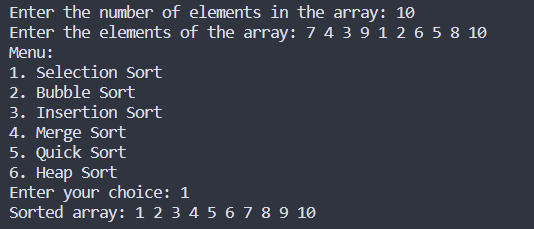
\includegraphics[width=0.55\textwidth]{Cycle_2/Outputs/Sort1.png}
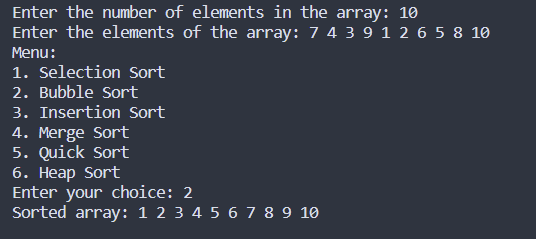
\includegraphics[width=0.55\textwidth]{Cycle_2/Outputs/Sort2.png}
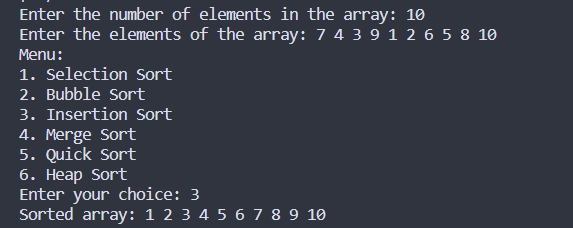
\includegraphics[width=0.55\textwidth]{Cycle_2/Outputs/Sort3.png}
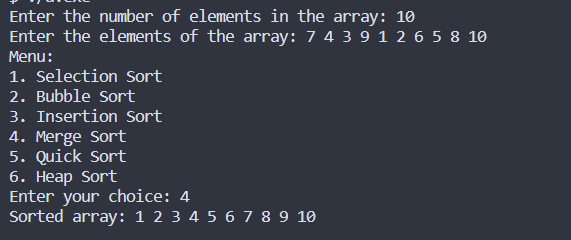
\includegraphics[width=0.55\textwidth]{Cycle_2/Outputs/Sort4.png}
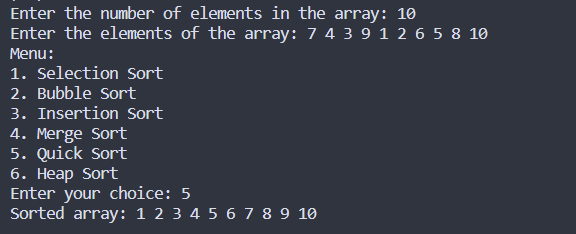
\includegraphics[width=0.55\textwidth]{Cycle_2/Outputs/Sort5.png}
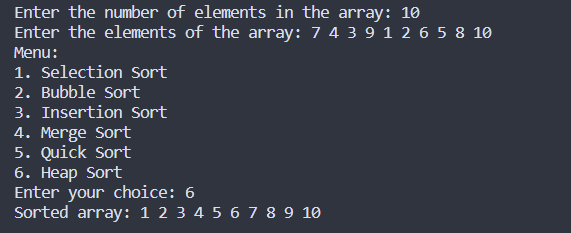
\includegraphics[width=0.55\textwidth]{Cycle_2/Outputs/Sort6.png}

\section{Result}
Sorting algorithms implemented. The program was executed and output verified.